\documentclass[tikz,border=6pt]{standalone}
\usepackage{amsmath}
\usepackage{tikz}
\usetikzlibrary{arrows.meta}

\begin{document}
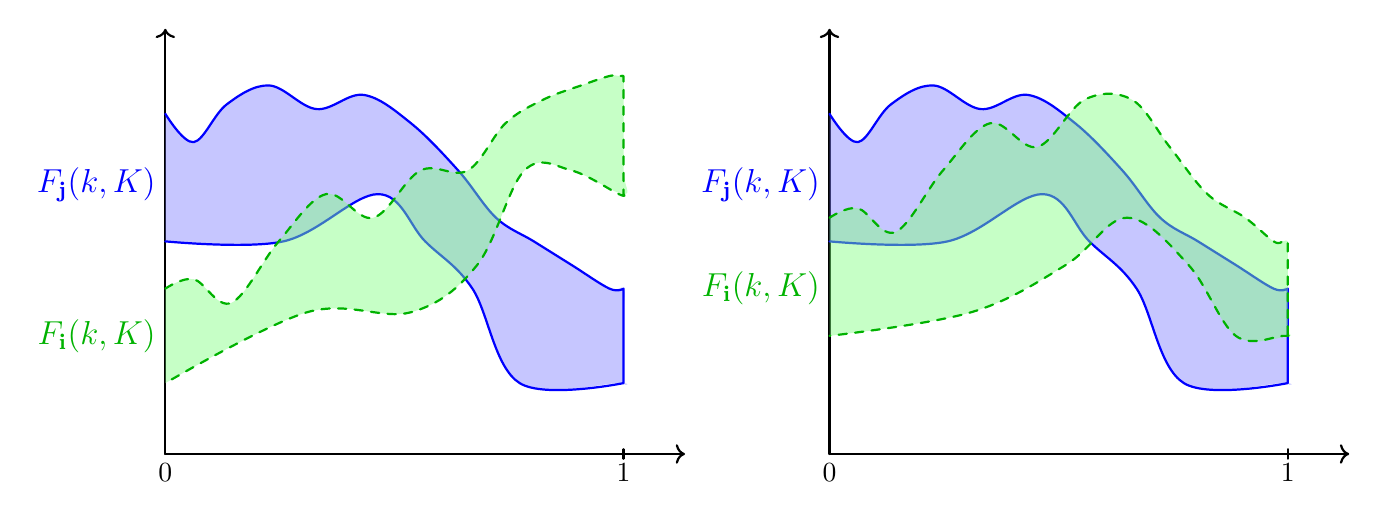
\begin{tikzpicture}[scale=6, line cap=round, line join=round]
		% Axes
		\draw[thick,->] (0,0) -- (1.1,0);
		\draw[thick,->] (0,0) -- (0,0.9);
		\draw[thick] (0.97,-0.01) -- (0.97,0.01);
		\node[below] at (0,0) {$0$};
		\node[below] at (0.97,0) {$1$}; % label before arrow
		
		% ===== BLUE region (20 points) =====
		% Order: start at left top -> along top to right top -> vertical down -> back along bottom to left bottom -> close
		\fill[blue!50, opacity=0.45]
		plot[smooth, tension=0.6] coordinates {
			(0.00,0.72) (0.06,0.66) (0.13,0.74) (0.22,0.78) (0.32,0.73)
			(0.42,0.76) (0.52,0.70) (0.62,0.60) (0.70,0.50) (0.78,0.45)
			(0.86,0.40) (0.94,0.35) (0.97,0.35) % right top
			(0.97,0.30) (0.97,0.20) (0.97,0.15) % right bottom (vertical segment)
			(0.96,0.15) (0.75,0.15) (0.65,0.35) (0.55,0.45) (0.45,0.55) (0.25,0.45)
			(0.00,0.45) % left bottom (vertical segment back to start)
		} -- cycle;
		% outline as single closed path (so the solid blue line follows the filled boundary)
		\draw[blue, thick]
		plot[smooth, tension=0.6] coordinates {
			(0.00,0.72) (0.06,0.66) (0.13,0.74) (0.22,0.78) (0.32,0.73)
			(0.42,0.76) (0.52,0.70) (0.62,0.60) (0.70,0.50) (0.78,0.45)
			(0.86,0.40) (0.94,0.35) (0.97,0.35)
		}
		-- (0.97,0.15)
		plot[smooth, tension=0.6] coordinates {
			(0.97,0.15) (0.75,0.15) (0.65,0.35) (0.55,0.45) (0.45,0.55) (0.25,0.45)
			(0.00,0.45)
		};
		
		% ===== GREEN region (20 points) =====
		\fill[green!50, opacity=0.45]
		plot[smooth, tension=0.6] coordinates {
			(0.00,0.35) (0.06,0.37) (0.14,0.32) (0.24,0.45) (0.34,0.55)
			(0.44,0.50) (0.54,0.60) (0.64,0.60) (0.72,0.70) (0.80,0.75)
			(0.88,0.78) (0.94,0.80) (0.96,0.80) (0.97,0.80) % right top
			(0.97,0.75) (0.97,0.60) (0.97,0.55) % right bottom (vertical segment)
			(0.86,0.60) (0.76,0.60) (0.66,0.40) (0.52,0.30) (0.30,0.30)
			(0.00,0.15) % left bottom
		} -- cycle;
		\draw[green!70!black, thick, dashed]
		plot[smooth, tension=0.6] coordinates {
			(0.00,0.35) (0.06,0.37) (0.14,0.32) (0.24,0.45) (0.34,0.55)
			(0.44,0.50) (0.54,0.60) (0.64,0.60) (0.72,0.70) (0.80,0.75)
			(0.88,0.78) (0.94,0.80) (0.96,0.80) (0.97,0.80)
		}
		-- (0.97,0.55)
		plot[smooth, tension=0.6] coordinates {
			(0.97,0.55) (0.96,0.55) (0.86,0.60) (0.76,0.60) (0.66,0.40) (0.52,0.30) (0.30,0.30)
			(0.00,0.15)
		};
		
		% Labels (colors roughly matching original)
		\node[blue, left] at (-0.0,0.57) {{\large $F_{\mathbf{j}}(k,K)$}};
		\node[green!70!black, left] at (-0.0,0.25) {{\large $F_{\mathbf{i}}(k,K)$}};

\begin{scope}[xshift=40]
		% Axes
\draw[thick,->] (0,0) -- (1.1,0);
\draw[thick,->] (0,0) -- (0,0.9);
\draw[thick] (0.97,-0.01) -- (0.97,0.01);
\node[below] at (0,0) {$0$};
\node[below] at (0.97,0) {$1$}; % label before arrow

% ===== BLUE region (20 points) =====
% Order: start at left top -> along top to right top -> vertical down -> back along bottom to left bottom -> close
\fill[blue!50, opacity=0.45]
plot[smooth, tension=0.6] coordinates {
	(0.00,0.72) (0.06,0.66) (0.13,0.74) (0.22,0.78) (0.32,0.73)
	(0.42,0.76) (0.52,0.70) (0.62,0.60) (0.70,0.50) (0.78,0.45)
	(0.86,0.40) (0.94,0.35) (0.97,0.35) % right top
	(0.97,0.30) (0.97,0.20) (0.97,0.15) % right bottom (vertical segment)
	(0.96,0.15) (0.75,0.15) (0.65,0.35) (0.55,0.45) (0.45,0.55) (0.25,0.45)
	(0.00,0.45) % left bottom (vertical segment back to start)
} -- cycle;
% outline as single closed path (so the solid blue line follows the filled boundary)
\draw[blue, thick]
plot[smooth, tension=0.6] coordinates {
	(0.00,0.72) (0.06,0.66) (0.13,0.74) (0.22,0.78) (0.32,0.73)
	(0.42,0.76) (0.52,0.70) (0.62,0.60) (0.70,0.50) (0.78,0.45)
	(0.86,0.40) (0.94,0.35) (0.97,0.35)
}
-- (0.97,0.15)
plot[smooth, tension=0.6] coordinates {
	(0.97,0.15) (0.75,0.15) (0.65,0.35) (0.55,0.45) (0.45,0.55) (0.25,0.45)
	(0.00,0.45)
};

% ===== GREEN region (20 points) =====
\fill[green!50, opacity=0.45]
plot[smooth, tension=0.6] coordinates {
	(0.00,0.50) (0.06,0.52) (0.14,0.47) (0.24,0.60) (0.34,0.70)
	(0.44,0.65) (0.54,0.75) (0.64,0.75) (0.72,0.65) (0.80,0.55)
	(0.88,0.50) (0.94,0.45) (0.96,0.45) (0.97,0.45) % right top
	(0.97,0.42) (0.97,0.27) (0.97,0.25) % right bottom (vertical segment)
	(0.86,0.25) (0.76,0.40) (0.63,0.50) (0.50,0.40) (0.30,0.30)
	(0.00,0.25) % left bottom
} -- cycle;
\draw[green!70!black, thick, dashed]
plot[smooth, tension=0.6] coordinates {
	(0.00,0.50) (0.06,0.52) (0.14,0.47) (0.24,0.60) (0.34,0.70)
	(0.44,0.65) (0.54,0.75) (0.64,0.75) (0.72,0.65) (0.80,0.55)
	(0.88,0.50) (0.94,0.45) (0.96,0.45) (0.97,0.45)
}
-- (0.97,0.25)
plot[smooth, tension=0.6] coordinates {
	(0.97,0.25) (0.96,0.25) (0.86,0.25) (0.76,0.40) (0.63,0.50) (0.50,0.40) (0.30,0.30)
	(0.00,0.25)
};

% Labels (colors roughly matching original)
\node[blue, left] at (-0.0,0.57) {{\large $F_{\mathbf{j}}(k,K)$}};
\node[green!70!black, left] at (-0.0,0.35) {{\large $F_{\mathbf{i}}(k,K)$}};
\end{scope}
		
\end{tikzpicture}
\end{document}